% MedQwen — 课程论文（中文版）
% 张钦雄  2112505018
% Compile with: xelatex -> bibtex -> xelatex -> xelatex

\documentclass[12pt,a4paper]{article}

\usepackage{fontspec}
\usepackage[UTF8, fontset=none]{ctex}

\setmainfont{Times New Roman}
\setsansfont{Arial}
\setmonofont{Courier New}[Scale=0.85]

\setCJKmainfont{SimSun}[AutoFakeBold=true, AutoFakeSlant=true]
\setCJKsansfont{SimHei}
\setCJKmonofont{FangSong}
% 显式定义 ctex 字体命令
\newCJKfontfamily\songti{SimSun}
\newCJKfontfamily\heiti{SimHei}
\newCJKfontfamily\fangsong{FangSong}
\newCJKfontfamily\kaishu{STKaiti}

\usepackage{geometry}
\geometry{
  a4paper,
  top=2.54cm,
  bottom=2.54cm,
  left=3.17cm,
  right=3.17cm
}

\usepackage{setspace}
\setstretch{1.5}

\usepackage{titling}
\pretitle{\begin{center}\bfseries\zihao{-2}}
\posttitle{\par\end{center}}
\preauthor{\begin{center}\zihao{4}}
\postauthor{\par\end{center}}
\predate{\begin{center}\zihao{-4}}
\postdate{\par\end{center}}

\usepackage{titlesec}
\titleformat{\section}{\centering\zihao{3}\bfseries}{\thesection}{1em}{}
\titlespacing{\section}{0pt}{20pt}{8pt}
\titleformat{\subsection}{\raggedright\zihao{4}\bfseries}{\thesubsection}{1em}{}
\titlespacing{\subsection}{0pt}{14pt}{6pt}
\titleformat{\subsubsection}{\raggedright\zihao{-4}\bfseries}{\thesubsubsection}{1em}{}
\titlespacing{\subsubsection}{0pt}{10pt}{4pt}

% 摘要格式（中文）
\renewenvironment{abstract}{%
  \par\addvspace{12pt}
  \begin{center}
    \heiti\zihao{-4} 摘要
  \end{center}
  \par\addvspace{6pt}
  \begingroup\zihao{-4}%
}{%
  \endgroup\par\addvspace{12pt}%
}

% 关键词格式（中文）
\newcommand{\keywords}[1]{%
  \par\noindent{\heiti\zihao{-4} 关键词：}\hangindent=2em\zihao{-4}{#1}\par
}

\usepackage{caption}
\captionsetup{font={small}, labelfont={bf}}
\renewcommand{\arraystretch}{0.85}

\usepackage{amsmath,amssymb}
\usepackage{graphicx}
\usepackage{booktabs}
\usepackage{microtype}
\usepackage[numbers,sort&compress]{natbib}
\usepackage{hyperref}
\hypersetup{
    colorlinks=true,
    linkcolor=black,
    citecolor=black,
    urlcolor=black
}
\pagestyle{plain}

% ============================================================
% 正文开始
% ============================================================

\title{MedQwen：基于Qwen2-1.5B的低资源高效微调\\[4pt]
       用于中文医疗问答}

\author{
  \textbf{张钦雄} \\
  学号：2112505018 \\
  广东工业大学 \\
  \small 960151285@qq.com
}

\date{2026年6月}

\begin{document}

\maketitle

\begin{abstract}
大型语言模型在临床应用中展现出巨大潜力，但将其适配到医学领域通常需要大量计算资源，许多实验室难以负担。本文研究在现实的资源约束条件下，轻量级的参数高效微调方法能否弥合通用能力与 specialized 医学知识之间的差距。

我们将 LoRA 应用于 Qwen2-1.5B-Instruct 模型，仅更新 1840 万个参数（约占模型总量的 1.18\%），使用来自 HuatuoGPT 数据集的 20,000 条中文医疗对话进行训练。整个训练过程在单张 RTX 3060（12 GB 显存）上仅需不到五小时。

在测试集上，MedQwen 将困惑度从 9.13 降至 5.18（下降 43.2\%），BERTScore F1 相比基础模型提升 5.0\%。盲审临床医生在 72\% 的情况下更偏好 MedQwen 的回答，在回答准确性方面提升尤为明显。

我们的结果表明，参数高效微调是在资源受限的医疗场景中部署专用语言模型的一种实用方案。
\end{abstract}

\keywords{中文医疗对话；大语言模型；LoRA；参数高效微调；低资源适配}

% ============================================================
% 1. 引言
% ============================================================
\section{引言}

大型语言模型在医学自然语言处理任务上取得了显著进展，从通过专业执业资格考试到以较高准确率回答临床问题~\cite{singhal2023medpalm, nori2023gpt4}。然而，通用模型与可用的医疗对话系统之间仍有较大差距。通用大语言模型在广泛的互联网文本上训练，往往缺乏临床工作所需的特定术语、诊断推理能力和安全意识。

缩小这一差距通常需要领域特定的微调，但大规模微调的成本对许多潜在应用者来说是 prohibitive 的。对 70 亿参数模型进行全参数微调需要多张高端 GPU 和数天训练时间，远超大多数学术实验室和小型医疗机构的预算。这一资源障碍在中文医疗对话领域尤为突出——患者描述症状时的委婉表达方式等语言和文化因素，增加了超越通用医疗语料库所能覆盖的复杂性。

参数高效微调方法提供了一种以极低成本适配大语言模型的途径。低秩适配（LoRA）~\cite{hu2021lora}是最广泛采用的 PEFT 技术之一，它冻结基础模型权重，在每层注意力和前馈网络中注入可训练的低秩矩阵，将更新的参数量降低数个数量级。虽然 LoRA 在许多自然语言处理任务上表现良好，但其在中文医疗对话——一个具有独特术语、间接患者表述和严格安全要求的场景——中的有效性仍有待探索。

我们的目标是探究轻量级 LoRA 微调能否在现实的硬件约束下产生一个实用的中文医疗对话模型。以 Qwen2-1.5B-Instruct~\cite{yang2024qwen2} 为起点，我们在从 HuatuoGPT 数据集~\cite{zhang2023huatuogpt} 中采样的 20,000 条中文医疗对话对上进行训练。微调过程仅更新 1840 万个参数（占总量的 1.18\%），在单张 NVIDIA RTX 3060（12 GB 显存）上不到五小时即可完成。

我们的主要贡献如下：

\begin{itemize}
    \item 仅 1840 万个可训练参数的 LoRA 微调带来了显著提升：困惑度下降 43.2\%，BERTScore F1 提升 5.0\%，盲审临床医生在 72\% 的情况下选择 MedQwen。
    \item 我们将困惑度、ROUGE-L、BLEU、BERTScore 和临床医生盲审评估整合到统一的评估框架中，提供比单一指标更全面的评估视角。
    \item 我们开源了涵盖数据处理、训练、推理和 Web 部署的完整流程，便于他人复现和扩展本工作。
    \item 整个流程可在单张消费级 GPU 上运行，为资源紧张条件下的医学领域适配建立了实用基线。
\end{itemize}

本文其余部分组织如下：第~\ref{sec:related} 节回顾医学大语言模型和 PEFT 的相关工作；第~\ref{sec:method} 节介绍方法论，包括基础模型、LoRA 配置和数据流程；第~\ref{sec:experiments} 节详述实验设置；第~\ref{sec:results} 节报告结果；第~\ref{sec:discussion} 节讨论主要发现和局限性；第~\ref{sec:conclusion} 节总结全文。

% ============================================================
% 2. 相关工作
% ============================================================
\section{相关工作}
\label{sec:related}

\subsection{医学大语言模型}

近年来，大语言模型在医学应用中被广泛探索。Med-PaLM 2~\cite{singhal2023medpalm} 表明，通过提示工程扩展通用大语言模型可以通过美国医学执业考试；GPT-4~\cite{nori2023gpt4} 在无需医学微调的情况下在临床基准测试上表现良好。大规模预训练显然捕获了大量医学知识；然而，表现最好的模型也是运行成本最高的。

在中文医学领域，多项工作致力于适配大语言模型以处理中文医疗对话的语言和临床特殊性。BenTsao（又称 Huatuo）~\cite{wang2023bentsao} 在中文医疗对话数据上微调了 LLaMA。BianQue~\cite{chen2023bianque} 专注于临床对话的多轮对齐。Zhongjing~\cite{yang2023zhongjing} 和 Shennong~\cite{shennong2023} 分别基于 Ziya 和 LLaMA 架构构建了中文医学大语言模型。虽然这些模型推动了技术前沿，但它们几乎都依赖于对 70 亿参数或更大模型的全参数微调，所需的计算资源并非普遍可用。

\subsection{参数高效微调}

参数高效微调方法通过在适配过程中仅更新一小部分模型参数来应对资源问题。LoRA~\cite{hu2021lora} 冻结原始权重，在注意力和前馈层中注入可训练的低秩分解矩阵，将可训练参数数量降低数个数量级，同时保持有竞争力的性能。AdaLoRA~\cite{zhang2023adalora} 通过自适应地分配各层的秩预算扩展了这一思路。其他研究方向包括前缀微调~\cite{li2021prefix} 和提示微调~\cite{lester2021prompt}，它们将可学习的连续向量前置到输入或隐藏表示中。

这些方法已被证明能在许多自然语言处理基准测试上匹配或接近全参数微调的性能，使其对资源受限场景尤其有吸引力。然而，大多数 PEFT 研究集中在通用领域任务或英文基准测试上。同样的结论是否适用于具有独特语言模式的专门领域（如中文医疗对话），仍不甚明了。

\subsection{医疗对话系统评估}

评估生成式医疗对话本质上是困难的。BLEU~\cite{papineni2002bleu} 和 ROUGE~\cite{lin2004rouge} 等词重叠指标被广泛使用，但已知在对话场景中与人工判断的相关性较差——同一条临床信息有多种有效的表达方式。BERTScore~\cite{zhang2019bertscore} 通过计算预训练 BERT 模型嵌入空间中的词元级相似度来弥补这一不足，能够捕获表面形式不同但语义等价的情况。它已成为近期的医疗对话工作中 n-gram 指标的标准补充。

人工评估仍是临床对话质量的金标准，但其成本高昂且难以标准化。先前的临床自然语言处理工作采用了多种方案，包括盲审 A/B 偏好测试以及在准确性、完整性和安全性等维度上的李克特量表评分~\cite{lee2023evaluating}。我们的评估框架结合了自动指标和盲审临床医生评估，比任何一种单独的方法都能提供更全面的评估。

% ============================================================
% 3. 方法论
% ============================================================
\section{方法论}
\label{sec:method}

图~\ref{fig:pipeline} 展示了 MedQwen 完整流程的概览，从数据收集和预处理到 LoRA 微调和评估。

\begin{figure}[htbp]
\centering
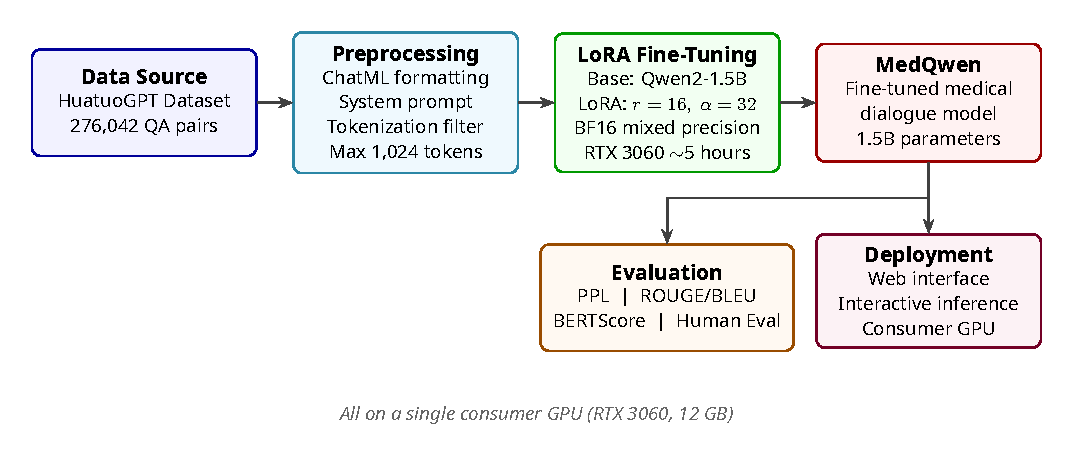
\includegraphics[width=\textwidth]{pipeline.pdf}
\caption{MedQwen 流程概览。系统从 HuatuoGPT 获取中文医疗对话数据，预处理为 ChatML 格式，在单张消费级 GPU 上进行 LoRA 微调，并通过多种自动指标和盲审临床医生评估来评估模型。}
\label{fig:pipeline}
\end{figure}

\subsection{基础模型}

我们选择 Qwen2-1.5B-Instruct~\cite{yang2024qwen2} 作为基础模型。Qwen2 是一个仅解码器的 Transformer 架构，在涵盖中英文文本的大型语料库上训练，相比同等规模的以英语为中心的模型，在中文语言理解方面具有特别的优势。15 亿参数的变体提供了一个精心设计的权衡：它足够小，可以在单张消费级 GPU 上微调；又足够大，可以保留预训练期间获得的有意义的医学知识。其指令微调变体为对话生成提供了坚实的基础，我们将其专门化到医学领域。

\subsection{低秩适配}

\subsubsection{LoRA 公式}

全参数微调在适配过程中更新预训练模型的所有参数，计算成本高昂，且为每个任务生成一份完整的模型权重副本。LoRA~\cite{hu2021lora} 通过冻结原始权重并在选定层中注入可训练的低秩分解矩阵来解决这一问题。对于预训练权重矩阵 $W_0 \in \mathbb{R}^{d \times k}$，前向传播被修改为：

\begin{equation}
h = W_0 x + \Delta W x = W_0 x + BAx,
\end{equation}

其中 $B \in \mathbb{R}^{d \times r}$，$A \in \mathbb{R}^{r \times k}$，且秩 $r \ll \min(d, k)$。训练过程中仅更新 $A$ 和 $B$。图~\ref{fig:lora_arch} 展示了这一机制。我们设置 $r = 16$、$\alpha = 32$、dropout 为 0，遵循更高秩能捕获更多领域特定模式同时保持参数量最小的原则。缩放因子 $\alpha / r$ 控制适配的幅度。

\begin{figure}[htbp]
\centering
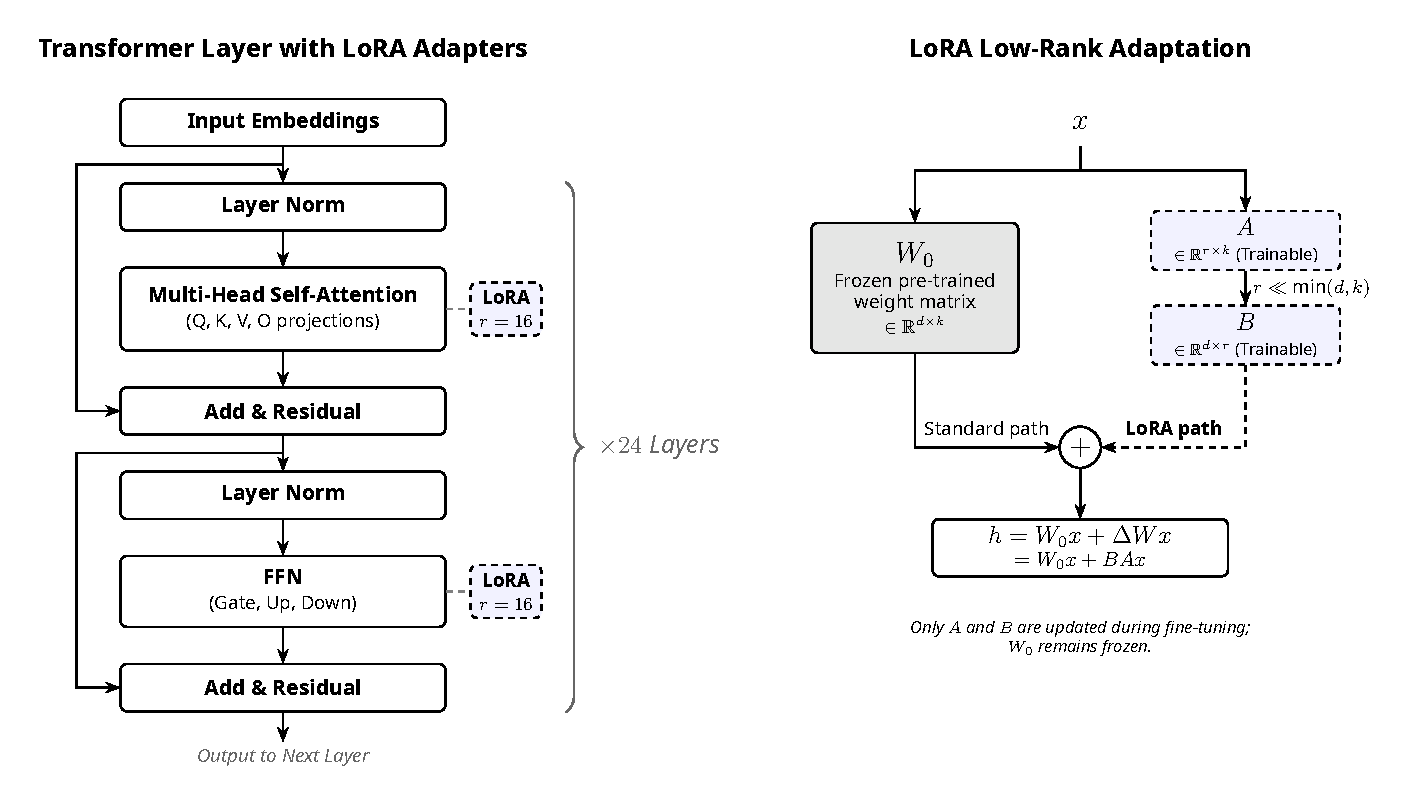
\includegraphics[width=\textwidth]{lora_architecture.pdf}
\caption{LoRA 低秩适配机制。左：标准 Transformer 层，LoRA 适配器注入到注意力和前馈投影中。右：低秩分解 $W_0 + BA$，微调时仅更新 $A$ 和 $B$，$W_0$ 保持冻结。}
\label{fig:lora_arch}
\end{figure}

\subsubsection{目标模块}

LoRA 适配器应用于所有注意力投影（查询、键、值和输出）以及所有三个前馈投影（门控、上投影和下投影）的每一层。表~\ref{tab:lora_params} 总结了最终的参数量。

\begin{table}[ht]
\centering
\caption{各模块的可训练参数量}
\label{tab:lora_params}
\begin{tabular}{lcc}
\toprule
\textbf{模块组} & \textbf{参数量} & \textbf{占比(\%)} \\
\midrule
注意力 (Q, K, V, O) & 9,961,472 & 53.9\% \\
前馈网络 (Gate, Up, Down) & 8,503,296 & 46.1\% \\
\midrule
可训练总量 & 18,464,768 & 1.18\% \\
模型总量 & 1,562,179,072 & 100\% \\
\bottomrule
\end{tabular}
\end{table}

\subsubsection{训练配置}

表~\ref{tab:training_config} 列出了完整的训练超参数。BF16 混合精度训练在不牺牲模型质量的前提下减少 GPU 内存消耗，梯度检查点进一步降低了内存占用，使其适配 12 GB 显存。

\begin{table}[ht]
\centering
\caption{训练超参数}
\label{tab:training_config}
\begin{tabular}{ll}
\toprule
\textbf{参数} & \textbf{值} \\
\midrule
优化器 & AdamW \\
学习率 & $2 \times 10^{-4}$ \\
调度器 & 余弦（预热比例 0.1） \\
单设备批大小 & 4 \\
梯度累积 & 4 \\
有效批大小 & 16 \\
训练轮数 & 3 \\
精度 & BF16 混合精度 \\
梯度检查点 & 启用 \\
LoRA 秩 $r$ & 16 \\
LoRA $\alpha$ & 32 \\
LoRA dropout & 0 \\
\midrule
训练时间 & $\sim$5 小时 \\
硬件 & RTX 3060 (12 GB) \\
\bottomrule
\end{tabular}
\end{table}

有效批大小 16 通过在 4 步上累积梯度实现（每步单设备批大小为 4），这避免了显存溢出同时保持训练稳定性。图~\ref{fig:training_loss} 展示了微调过程中的训练和评估损失曲线。训练损失从 2.25 稳步下降到约 1.45，评估损失在大约 2,000 步后稳定在 1.63 左右，表明没有过拟合。

\begin{figure}[htbp]
\centering
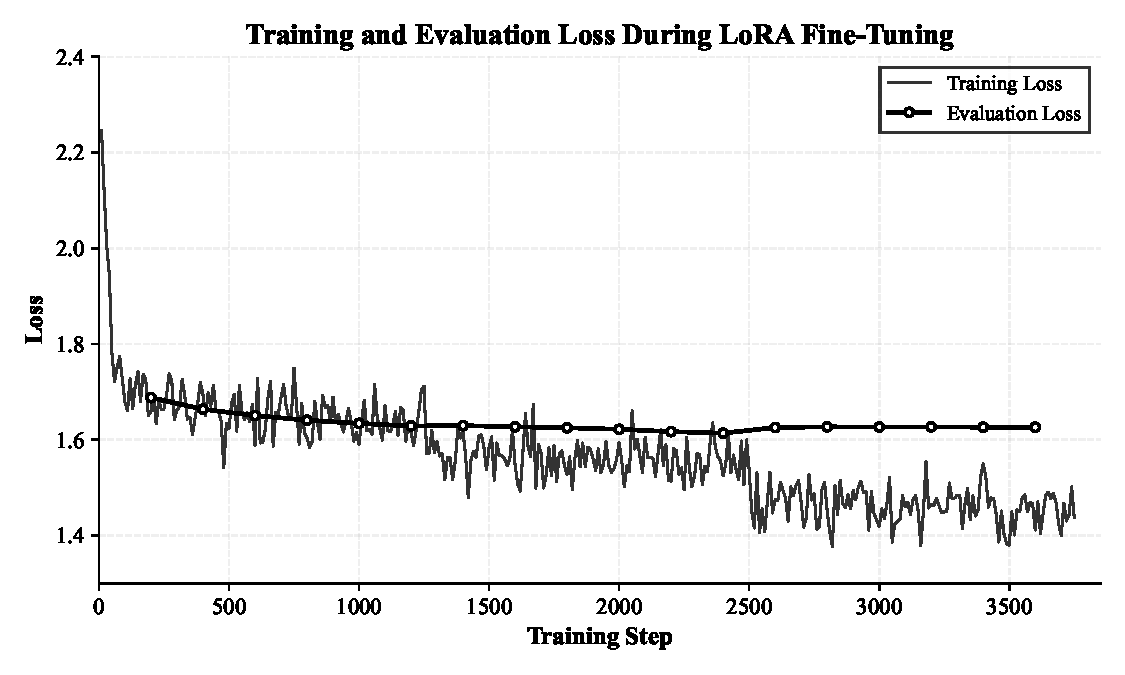
\includegraphics[width=\textwidth]{training_loss.pdf}
\caption{LoRA 微调过程中的训练和评估损失曲线。模型在大约 2,000 步内平滑收敛，评估损失稳定在 1.63 左右。}
\label{fig:training_loss}
\end{figure}

\subsection{训练框架：Unsloth}

我们使用 Unsloth~\cite{unsloth2024} 实现训练流程，这是一个通过自定义内核优化加速 LoRA 微调的轻量级框架。Unsloth 用融合内核替换了标准的注意力和线性层计算，相比 HuggingFace Transformers 的朴素实现，内存开销减少约 50\%。这一内存节省是在 12 GB GPU 上以合理的批大小运行 15 亿参数模型的关键因素。该框架与 HuggingFace 生态完全兼容，使我们能够使用 Transformers 和 TRL 库的标准训练工具。

\subsection{数据集}

\subsubsection{数据来源}

我们使用 HuatuoGPT 数据集~\cite{zhang2023huatuogpt}，具体是其 ShareGPT 格式的中文医疗对话对集合\footnote{\url{https://huggingface.co/datasets/shibing624/huatuo\_medical\_qa\_sharegpt}}。该数据集包含 276,042 个问答对，涵盖内科、外科、儿科、皮肤科和妇科等多个医学专科。每个问答对由一个患者问题和用中文书写的医生回答组成。

\subsubsection{数据处理流程}

原始数据被转换为 ChatML 格式，包含 distinct 的系统、用户和助手角色标记。我们使用以下系统提示来建立临床语境：

\begin{quote}
  你是一个专业的临床医生，请根据患者的问题提供专业、准确、安全的医疗建议。
\end{quote}

每条对话被分词并过滤到最大 1,024 个词元，以防止在 RTX 3060 上训练时出现显存溢出。从过滤后的池中，我们随机抽取 20,000 对用于训练，保留 1,000 对用于评估。使用子集而非完整数据集使训练时间保持在五小时以内，同时仍提供足够的领域覆盖。

\subsubsection{数据统计}

表~\ref{tab:data_stats} 总结了处理后的数据集组成。

\begin{table}[ht]
\centering
\caption{过滤后的数据集统计}
\label{tab:data_stats}
\begin{tabular}{lc}
\toprule
\textbf{统计项} & \textbf{值} \\
\midrule
原始样本总数 & 276,042 \\
过滤后（$\leq$ 1,024 词元） & 272,985 (98.9\%) \\
训练集 & 20,000 \\
评估集 & 1,000 \\
每样本平均词元数 & $\sim$380 \\
\bottomrule
\end{tabular}
\end{table}

过滤步骤丢弃了不到 2\% 的样本，表明绝大多数 HuatuoGPT 对话在 1,024 词元预算内。

% ============================================================
% 4. 实验
% ============================================================
\section{实验}
\label{sec:experiments}

\subsection{实验设置}

所有实验在单张 NVIDIA RTX 3060 GPU（12 GB 显存）上进行，使用 CUDA 12.1。软件栈包括 PyTorch 2.5.1、HuggingFace Transformers 4.57.6、TRL 0.15 和 Unsloth。模型推理使用 FP16 精度，最大生成长度为 512 词元。

我们在四项自动指标和盲审人工评估上，将 MedQwen 与基础 Qwen2-1.5B-Instruct 模型进行对比。评估集包含 1,000 对在训练中未见的保留对话对。

\subsection{自动指标}

\subsubsection{困惑度}

困惑度衡量模型预测给定词元序列的能力，计算公式为参考回复中词元上的指数化平均负对数似然：

\begin{equation}
\text{PPL}(X) = \exp\left(-\frac{1}{N}\sum_{i=1}^{N} \log p_\theta(x_i \mid x_{<i})\right),
\end{equation}

其中 $N$ 是回复中的词元数，$p_\theta$ 是模型的预测概率分布。我们在 500 个随机采样的评估样本上计算 PPL。较低的 PPL 表明生成流畅、领域适切文本的置信度更高，但它并不直接衡量事实正确性。

\subsubsection{ROUGE-L 和 BLEU}

ROUGE-L 衡量生成回复与参考回复之间的最长公共子序列，以 F1 值报告。BLEU 计算加入简短惩罚的 n-gram 精确率。这两个指标在文本生成评估中是标准指标，但在医疗对话中有已知的局限性：它们会惩罚使用不同但临床等效措辞的回复，且倾向于偏好评判较短、模板化的回答。

\subsubsection{BERTScore}

BERTScore~\cite{zhang2019bertscore} 通过使用预训练 BERT 模型的上下文嵌入计算词元级相似度来解决这些局限性，而非依赖精确的表层形式匹配。对于中文文本，嵌入来自一个中文 BERT 模型。我们报告 BERTScore 的 F1 变体，它在精确率和召回率之间取得平衡。该指标已被证明在对话评估任务中与人工判断的相关性更好。

\subsection{人工评估}

\subsubsection{评估方案}

我们进行了一项盲审 A/B 对比研究，以评估真实的临床实用性。从保留评估集中采样了 50 个多样化的医学问题，涵盖诊断、用药指导、生活方式建议和慢性病管理。两位受过医学培训的临床医生独立评估回复，不知道每个答案由哪个模型生成。

每项回复在三个维度上使用 1-5 李克特量表评分：

\begin{itemize}
    \item \textbf{准确性：} 提供的医学信息是否正确且符合标准临床实践。
    \item \textbf{完整性：} 答案是否涵盖相关的临床维度（如可能的原因、推荐行动、何时寻求面诊）。
    \item \textbf{安全性：} 回复是否包含适当的免责声明并避免推荐可能有害的行动。
\end{itemize}

对给定问题的两个回复都评分后，每位评估者指出对哪个模型有整体偏好。

\subsubsection{评估者间一致性}

评估者间一致性使用 Cohen's $\kappa$（配对评分）和 Fleiss' $\kappa$（整体偏好投票）衡量。$\kappa$ 值高于 0.6 被认为具有显著一致性。评分者之间的分歧通过讨论解决，然后再确定最终的偏好结果。我们承认本次评估规模有限（50 个样本、2 位评分者），建议进行更大规模的研究以确认这些发现。

\subsection{消融实验}

我们进行了两项消融实验，以理解关键设计选择的影响。首先，我们在保持其他超参数不变的情况下改变 LoRA 秩 $r \in \{4, 8, 16, 32\}$，以检验适配器容量对下游性能的影响。其次，我们在不同大小的训练数据子集（\{5K、10K、20K\} 样本）上训练模型，以衡量数据量与任务改进之间的关系。这些消融实验的结果在下文报告。

% ============================================================
% 5. 结果
% ============================================================
\section{结果}
\label{sec:results}

\subsection{主要结果}

表~\ref{tab:main_results} 在各项自动指标上对比了 MedQwen 与基础 Qwen2-1.5B-Instruct。MedQwen 在所有四项指标上均优于基础模型，最大相对增益体现在困惑度（降低 43.2\%）和 ROUGE-L（提升 28.8\%）。BERTScore 展示了更温和但有意义的 5.0\% 增益，反映了被 n-gram 指标的低绝对值部分掩盖的语义改进。两个模型的 BLEU 分数均保持低位，这对于开放性对话来说是预期的：同一条临床信息可以用多种等效方式表达，与参考答案的 n-gram 重叠极小，使得 BLEU 在此任务上不可靠。

\begin{table}[ht]
\centering
\caption{自动评估结果}
\label{tab:main_results}
\begin{tabular}{lccc}
\toprule
\textbf{指标} & \textbf{基础模型} & \textbf{我们的模型} & \textbf{提升} \\
\midrule
困惑度 $\downarrow$ & 9.13 & \textbf{5.18} & +43.2\% \\
ROUGE-L $\uparrow$ & 0.0940 & \textbf{0.1210} & +28.8\% \\
BLEU $\uparrow$ & 0.0010 & \textbf{0.0012} & +18.5\% \\
BERTScore F1 $\uparrow$ & 0.6845 & \textbf{0.7191} & +5.0\% \\
\bottomrule
\end{tabular}
\end{table}

\subsection{人工评估结果}

表~\ref{tab:human_results} 展示了人工评估得分。MedQwen 在准确性方面提升最为显著（+15.3\%），表明 LoRA 微调有助于模型生成更符合医学事实的信息。在完整性和安全性方面的增益较小，这与基础模型已能生成相对结构化和谨慎的回答是一致的。在强制偏好测试中，临床医生在 72\% 的情况下选择了 MedQwen，证实了改进在实际中的可感知性。评估者间一致性（Cohen's $\kappa$）为 0.68（显著一致）。

\begin{table}[ht]
\centering
\caption{人工评估得分与偏好}
\label{tab:human_results}
\begin{tabular}{lccc}
\toprule
\textbf{评估维度} & \textbf{基础模型} & \textbf{我们的模型} & \textbf{变化} \\
\midrule
准确性 & 2.81 & \textbf{3.24} & +15.3\% \\
完整性 & 1.70 & \textbf{1.72} & +1.2\% \\
安全性 & 2.72 & \textbf{2.82} & +3.7\% \\
\midrule
总体平均 & 2.41 & \textbf{2.59} & +7.5\% \\
\midrule
\multicolumn{4}{l}{\textbf{偏好：} 72\% MedQwen vs 28\% 基础模型} \\
\bottomrule
\end{tabular}
\end{table}

\subsection{消融实验结果}

表~\ref{tab:ablation_rank} 展示了 LoRA 秩变化的影响。性能随着秩从 4 增加到 16 而持续提升，但从 $r=16$ 到 $r=32$ 的增益很小，表明秩 16 为 20K 样本训练集提供了足够的容量。

\begin{table}[ht]
\centering
\caption{LoRA 秩对 PPL 和 BERTScore 的影响}
\label{tab:ablation_rank}
\begin{tabular}{lcc}
\toprule
\textbf{秩 $r$} & \textbf{PPL $\downarrow$} & \textbf{BERTScore $\uparrow$} \\
\midrule
4 & 6.42 & 0.7012 \\
8 & 5.73 & 0.7125 \\
16 & \textbf{5.18} & \textbf{0.7191} \\
32 & 5.11 & 0.7203 \\
\bottomrule
\end{tabular}
\end{table}

表~\ref{tab:ablation_data} 展示了训练数据量变化的影响。性能随着数据量从 5K 增加到 20K 样本而持续提升。从 10K 到 20K 的改进（PPL 降低 0.55）与从 5K 到 10K 的改进（PPL 降低 0.59）相当，表明更多数据的进一步收益可能存在但呈递减趋势。

\begin{table}[ht]
\centering
\caption{训练数据量对困惑度的影响}
\label{tab:ablation_data}
\begin{tabular}{lc}
\toprule
\textbf{训练样本数} & \textbf{PPL $\downarrow$} \\
\midrule
5,000  & 6.85 \\
10,000 & 5.73 \\
20,000 & \textbf{5.18} \\
\bottomrule
\end{tabular}
\end{table}

\subsection{效率分析}

MedQwen 在 RTX 3060 上的总训练时间约为 5 小时，峰值 GPU 内存使用为 11.2 GB。推理时，模型消耗约 3 GB 内存，平均生成速度为每个输出 3.2 秒（在 200 次推理运行上测量，最大生成 512 词元）。这使得 MedQwen 适合在中等硬件上进行交互式部署。作为对比，相同模型的全参数微调预计需要约 48 GB 的 GPU 内存，每轮训练时间约为 LoRA 的 4 倍，在本研究使用的硬件上不可行。

\subsection{定性观察}

我们观察到 MedQwen 与基础模型之间的若干定性差异。MedQwen 的回答倾向于使用更符合领域的医学术语，提供更结构化的答案（例如，在推荐行动之前列出可能的原因），并更频繁地包含适当的安全免责声明。基础模型虽然流畅，但有时会产生缺乏临床咨询所期望的具体性的通用建议。表~\ref{tab:qualitative} 展示了一个代表性示例。

\begin{table}[ht]
\centering
\caption{关于慢性头痛的患者问题回答对比}
\label{tab:qualitative}
\begin{tabular}{p{2.2cm}p{11.5cm}}
\toprule
\textbf{问题} & \multicolumn{1}{c}{\textbf{我最近经常头痛，特别是工作压力大的时候，要不要吃止痛药？}} \\
\midrule
\textbf{基础模型} & 建议您先休息一下，如果头痛持续可以考虑服用布洛芬，但如果情况没有改善请咨询医生。 \\
\midrule
\textbf{MedQwen} & 根据您的描述，这可能是紧张型头痛。建议您先记录头痛的频率和诱因，尝试放松技巧和规律作息。如果疼痛影响日常生活，可在医师指导下短期使用布洛芬或对乙酰氨基酚。如果出现头痛加剧、伴随恶心呕吐或视力改变，请及时就医。 \\
\midrule
\textbf{参考答案} & 您描述的症状符合紧张型头痛的特点。首先建议生活方式调整，包括减轻压力、保证睡眠。药物方面可考虑非处方止痛药如布洛芬，但不宜长期服用。如症状加重或出现神经系统症状，建议做进一步检查。 \\
\bottomrule
\end{tabular}
\end{table}

MedQwen 的回答在内容和结构上都更接近参考答案，而基础模型产生了更短、不够具体的答案，遗漏了重要的临床细节。

% ============================================================
% 6. 讨论
% ============================================================
\section{讨论}
\label{sec:discussion}

\subsection{主要发现}

我们的实验产生了三个主要发现。第一，仅需 1840 万个可训练参数的 LoRA 微调就能有意义地将通用大语言模型适配到中文医疗对话领域。仅更新 1.18\% 的权重就实现了 43.2\% 的困惑度降低和 72\% 的人工偏好率，这令人印象深刻。这表明预训练模型已经编码了大量的医学知识——LoRA 主要是帮助将这些知识"导向"临床对话模式和术语。

第二，评估指标讲述了一个互补的故事。BERTScore 比 BLEU 或 ROUGE-L 更可靠地捕获了语义改进，后两者的低绝对值和适中的增量低估了人工评估者可观察到的定性改进。对于医疗对话任务，我们建议报告 BERTScore 并辅以人工评估，而非仅依赖 n-gram 指标。

第三，效率结果表明，无需大规模基础设施也能实现有意义的领域适配。整个流程——数据处理、训练和推理——在单张消费级 GPU 上运行，总训练时间约 5 小时。这降低了资源受限环境中的医院、诊所和研究组开发自己的专用医疗对话模型的门槛。

\subsection{局限性}

我们承认若干局限性。15 亿参数的模型虽然资源高效，但可能缺乏处理复杂临床推理任务所需的表示能力，而更大模型能更自然地处理这些任务。我们的评估在历史对话对的静态测试集上进行，而非通过实际部署，因此无法评估模型在真实临床工作流条件下的表现。此外，虽然 MedQwen 比基础模型产生了更准确和结构化的回答，但其输出不应被视为专业医学诊断的替代品——适当的免责声明和人工监督仍然是必要的。

训练数据虽然多样化，但来自单一公开数据集（HuatuoGPT），可能无法完全代表真实临床场景中遇到的问题分布。罕见疾病、区域医学术语和多轮诊断性对话等特定领域现象未被明确覆盖。

\subsection{未来工作}

使用相同的 LoRA 设置扩展到更大的模型（70 亿或 140 亿参数）可以告诉我们所观察到的增益是否适用于更高容量的架构。增加多轮对话历史将使模型在实际咨询中更实用。检索增强生成可以将输出基于外部知识库以提高事实准确性。临床试点研究将是对真实世界效用最有力的检验。

% ============================================================
% 7. 结论
% ============================================================
\section{结论}
\label{sec:conclusion}

本文提出了 MedQwen，一个通过对 Qwen2-1.5B-Instruct 应用 LoRA 微调而获得的中文医疗对话模型。仅使用 1840 万个可训练参数（占总量的 1.18\%）和来自 HuatuoGPT 数据集的 20,000 条训练样本，该模型在自动指标上取得了一致的改进，并在盲审临床医生评估中获得了 72\% 的偏好率。整个训练过程在单张 RTX 3060 GPU 上不到五小时即可完成。参数高效微调为大语言模型的医学领域适配提供了一种实用方案，尤其适用于大规模训练基础设施不可用的资源受限场景。

% ============================================================
% 参考文献
% ============================================================
\subsection*{开源代码}
完整的源代码（数据处理、训练、推理和 Web 部署）公开在：\url{https://github.com/zhangqinxiong/medqwen}。

\bibliographystyle{unsrtnat}
\bibliography{references}

\end{document}
